\documentclass[border=4pt]{standalone}
\usepackage{mathptmx}
\usepackage{tikz}
\usetikzlibrary{positioning,arrows.meta,calc}
\definecolor{frozenfill}{HTML}{F2F2F2}\definecolor{frozenline}{HTML}{8C8C8C}
\definecolor{trainfill}{HTML}{F7E3D3}\definecolor{trainline}{HTML}{B5652B}
\definecolor{salfill}{HTML}{E1E9F3}\definecolor{salline}{HTML}{4C72B0}
\tikzset{
  blk/.style={draw, rounded corners=1.5pt, line width=0.5pt, minimum width=45mm, text width=43mm, minimum height=10.5mm, align=center, font=\small},
  frozen/.style={blk, fill=frozenfill, draw=frozenline},
  trained/.style={blk, fill=trainfill, draw=trainline},
  sal/.style={blk, fill=salfill, draw=salline},
  arr/.style={-{Stealth[length=2.2mm]}, line width=0.5pt},
  lab/.style={font=\small\bfseries, anchor=east},
  sub/.style={font=\footnotesize\itshape}
}
\begin{document}
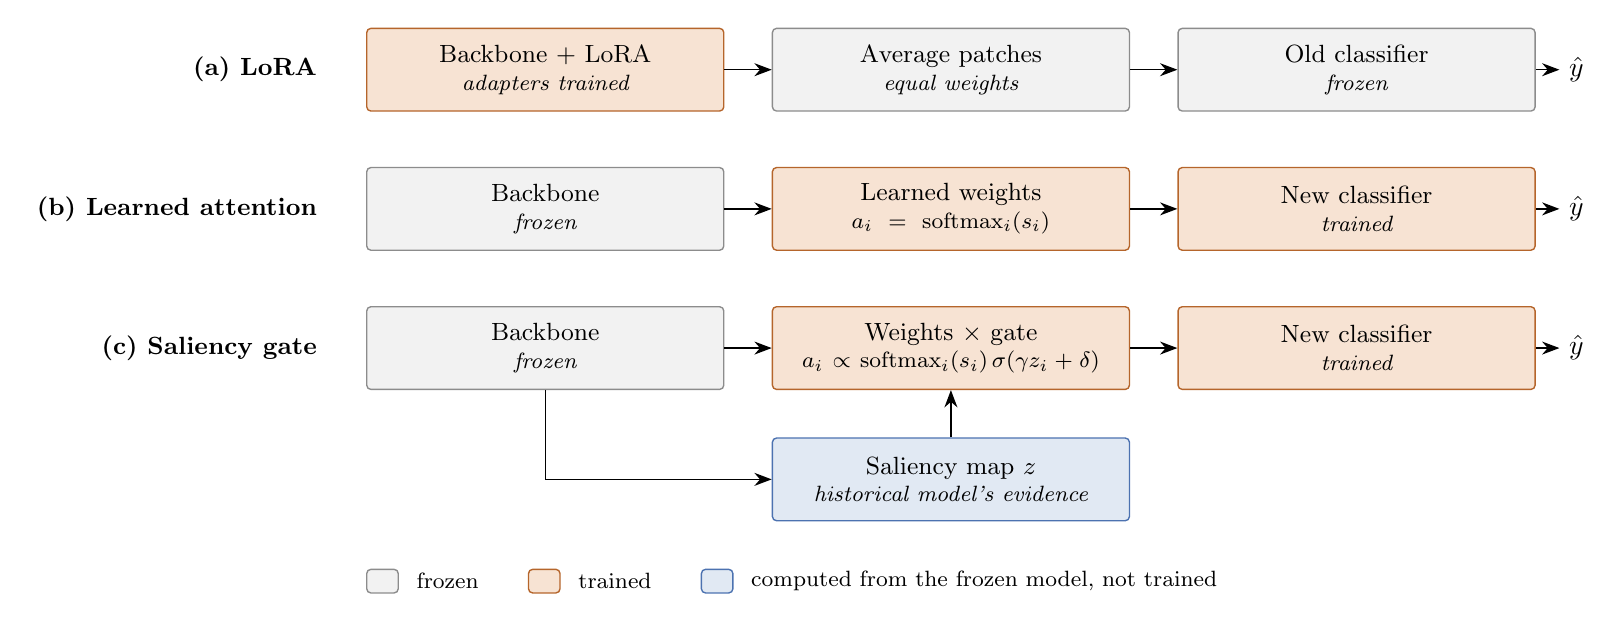
\begin{tikzpicture}[node distance=7mm and 6mm]
% (a) LoRA
\node[trained] (a1) {Backbone + LoRA\\[-1pt]{\footnotesize\itshape adapters trained}};
\node[frozen, right=of a1] (a2) {Average patches\\[-1pt]{\footnotesize\itshape equal weights}};
\node[frozen, right=of a2] (a3) {Old classifier\\[-1pt]{\footnotesize\itshape frozen}};
\node[right=3mm of a3] (ya) {$\hat{y}$};
\node[lab, left=5mm of a1] {(a) LoRA};
\draw[arr] (a1) -- (a2); \draw[arr] (a2) -- (a3); \draw[arr] (a3) -- (ya);
% (b) learned attention
\node[frozen, below=of a1] (b1) {Backbone\\[-1pt]{\footnotesize\itshape frozen}};
\node[trained, below=of a2] (b2) {Learned weights\\[-1pt]{\footnotesize $a_i=\mathrm{softmax}_i(s_i)$}};
\node[trained, below=of a3] (b3) {New classifier\\[-1pt]{\footnotesize\itshape trained}};
\node[right=3mm of b3] (yb) {$\hat{y}$};
\node[lab, left=5mm of b1] {(b) Learned attention};
\draw[arr] (b1) -- (b2); \draw[arr] (b2) -- (b3); \draw[arr] (b3) -- (yb);
% (c) saliency gate
\node[frozen, below=of b1] (c1) {Backbone\\[-1pt]{\footnotesize\itshape frozen}};
\node[trained, below=of b2] (c2) {Weights $\times$ gate\\[-1pt]{\footnotesize $a_i\propto\mathrm{softmax}_i(s_i)\,\sigma(\gamma z_i+\delta)$}};
\node[trained, below=of b3] (c3) {New classifier\\[-1pt]{\footnotesize\itshape trained}};
\node[right=3mm of c3] (yc) {$\hat{y}$};
\node[lab, left=5mm of c1] {(c) Saliency gate};
\draw[arr] (c1) -- (c2); \draw[arr] (c2) -- (c3); \draw[arr] (c3) -- (yc);
\node[sal, below=6mm of c2] (z) {Saliency map $z$\\[-1pt]{\footnotesize\itshape historical model's evidence}};
\draw[arr] (z) -- (c2);
\draw[arr] (c1.south) |- (z.west);
% legend
\node[frozen, minimum width=4mm, text width=, minimum height=3mm, anchor=north west] (l1) at ($(z.south -| c1.west)+(0,-6mm)$) {};
\node[right=1mm of l1, font=\footnotesize] (t1) {frozen};
\node[trained, minimum width=4mm, text width=, minimum height=3mm, right=5mm of t1] (l2) {};
\node[right=1mm of l2, font=\footnotesize] (t2) {trained};
\node[sal, minimum width=4mm, text width=, minimum height=3mm, right=5mm of t2] (l3) {};
\node[right=1mm of l3, font=\footnotesize] {computed from the frozen model, not trained};
\end{tikzpicture}
\end{document}
